\fancyhf{}
\fancyfoot[L]{\textbf{ECEN 4638--T.D. Murphey}}
\fancyfoot[R]{\textbf{Lab \#7}}
\fancyfoot[C]{\vspace{.2in}\thepage}

\chapter{Lab \#7: State Space Compensator Design}

\begin{center}  \textbf{Objective}
\end{center}

The purpose of this lab is to expose you to state space design techniques.  In
particular, you will use LQR techniques to design controllers and estimators.
Because you are now all largely familiar with LabVIEW, the description of this
lab will be kept rather brief.  However, keep in mind that this is nevertheless
a reasonably long lab\textendash don't put off the work until the second week!




\vspace{.2in}

\begin{center} \textsc{Note that this lab will be the last lab.}
\end{center}

\begin{center} \textbf{Warning:} 
\end{center}

As usual, please always run the ECP unit with someone holding the power button,
in case something happens to go wrong.

\newpage
\section{Pre-Lab Tasks}
Read this entire document before starting the lab.  
\section{Tasks}

\begin{enumerate}
\item The code that you will see will be found in \emph{students-simulation.vi,
    students-hardware.vi}, and \emph{students-estimator.vi}.  You will only need
  to edit the mathscript in \emph{students-simulation.vi} and
  \emph{students-estimator.vi}.
\item Note that you will \emph{only} change things in MathScript in this lab.
  Please do not change any of the graphical LabVIEW code except for rewiring the
  diagram to change full state feedback to estimated state feedback (as seen in
  Fig.\ref{fig-SSsim}).
\item Lastly, you will be given values for $c_{1,2,3}$ and $k_{1,2}$ for each
  torsional disk system.  Also, the hardware gain is now calculated within the
  code\textendash you don't need to address it.
\end{enumerate}



\subsection{Task \#1--State Space simulation}

\noindent \textbf{Task:}  Copy the folder {\tt state-space} from {\tt Desktop/ITLL Modules/ECEN Control Systems} to your Z: drive.


\noindent \textbf{Task:}  In \emph{students-simulation.vi}, replace the
second-order model with your model of the torsional disk system.  In
\emph{students-estimator.vi}, change the state feedback gain $K$ (near ``[MARKER
1]'') to be the appropriate length vector (e.g., it should match the dimension
of the state model) made up of zeros.  On the last line (near ``[MARKER 3]''),
set ``Nbar=1''\textendash this will allow you to track a reference input.  (This hack will
allow your code to compile, though there will be some errors due to the LQR
control and estimation calculations not matching the dimension of $K$.  You will
learn by next week what Nbar is and how to compute the controller, estimator,
and Nbar without errors.)

\noindent \textbf{Task:}  Simulate some open loop
response (using the top disk as the output) with nontrivial initial condition to
verify that your model is functioning properly.

\subsection{Task \#2--Controller Design}

Now that you have a model working, you should not need to change the
\emph{student-simulation.vi} file any more.  Instead, everything else should
occur within the \emph{student-estimator.vi} file, where both the controller and
estimator are designed.  First you will design a state-space controller for
stabilizing the top disk, then you will design a state-space estimator.  For the
controller, you should assume you have access to full state feedback\textendash\emph{make
  sure the block diagram reflects this}.

\noindent \textbf{Task:}  Implement a proportional controller and a PD
controller in state space form.  (I.e., You will have to replace your $K$ of
zeros with your own definition of $K$ that implements a PD control law.)
Simulate the closed loop response.  Is it sensitive to changes in system
parameters?  Disable the reference input and study your controller's response to 
initial conditions only by setting ``Nbar=0'' in \emph{students-estimator.vi}.

\begin{center} \textsc{This is probably a good stopping point for the first
    week.  However, you should have done most of the simulation components of
    this lab by the next time you meet.}
\end{center}


\noindent \textbf{Task:}  Design a controller using LQR (``lqr()'' in
MATLAB/MathScript)) that keeps the total control effort for a $1 rad$ step
response less than $2 Nm$ with a rise time of $t_r<0.75s$, overshoot $M_p<25\%$,
$e_{ss}<5\%$, and settle time $t_s<2s$.  To track a reference, you will need to
comment out the ``[MARKER 3]'' line so that Nbar is not disabled.  



\subsection{Task \#3--Estimator Design}

\noindent \textbf{Task:}  Rewire the simulation so that it is using estimated
state for purposes of control calculation, not the actual state.

\noindent \textbf{Task:}  Using the top disk as the output, design a state
estimator by placing the poles at desired locations using the command
``place()''.

\noindent \textbf{Task:} Simulate the system using your controller and the
estimated state.  Is your performance as good?  (You will have to comment out the
line at ``[MARKER 2]''.)

\noindent \textbf{Task:}  Using the formula for the controller $C(s)$ given
controller $K$
and estimator $L$, calculate the  phase margin and gain margin of your system?

\noindent \textbf{Task:}  Does your controller still work when you vary
parameters somewhat?  If it does, you need to iterate!

\subsection{Task \#4--Hardware Test}

\noindent \textbf{Task:}  If you are confident that your controller is working
properly in simulation, verify it in hardware.  This can be done using
\emph{students-hardware.vi}.  Set the hardware gain for your plant in the VI's 
wiring diagram and run it\textendash it will reference the
\emph{students-estimator.vi} you have already created.

\noindent \textbf{Task:}  What happens if you change the sample rate from $200
Hz$ to $500 Hz$?  to $1000 Hz$?  Why?



         

\noindent Remember, if you get stuck on some part of the lab, ask your
classmates, the TA, or myself.

\newpage

\begin{figure}[h!]
\centering
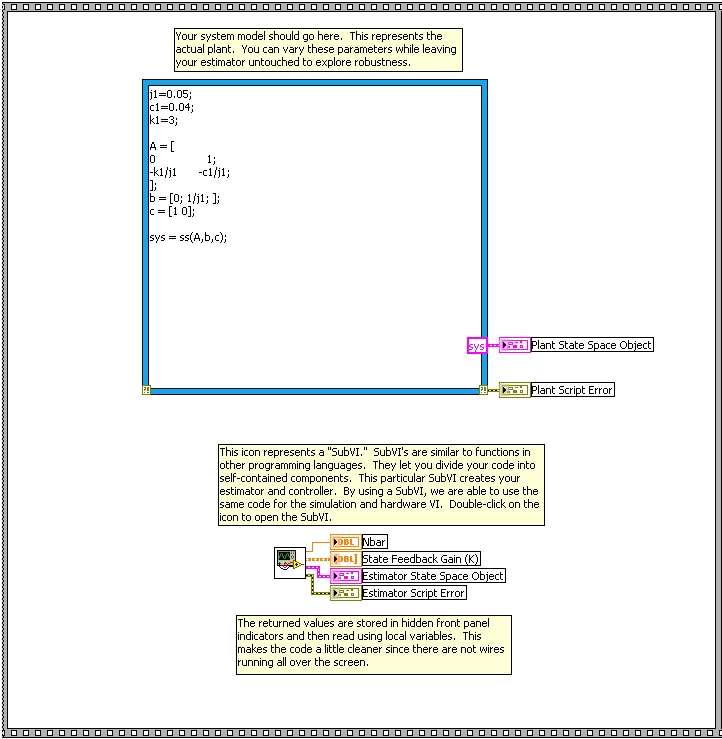
\includegraphics[width=6in]{statedomain/statespacesim1}
\caption{System Model}
\label{fig-SSsystemmodel}
\end{figure}

\begin{figure}[h!]
\centering
\rotatebox{90}{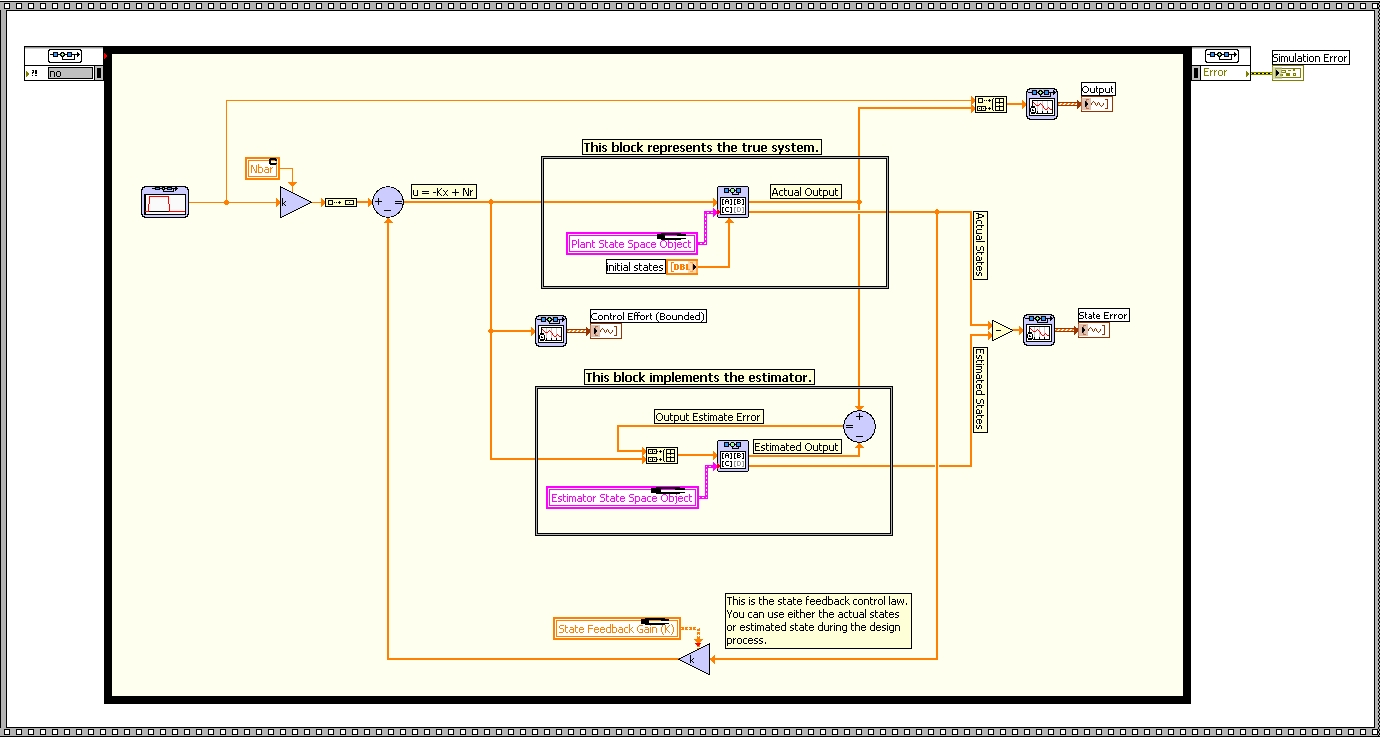
\includegraphics[width=9in]{statedomain/statespacesim2}}
\caption{State Space Simulation}
\label{fig-SSsim}
\end{figure}


\begin{figure}[h!]
\centering
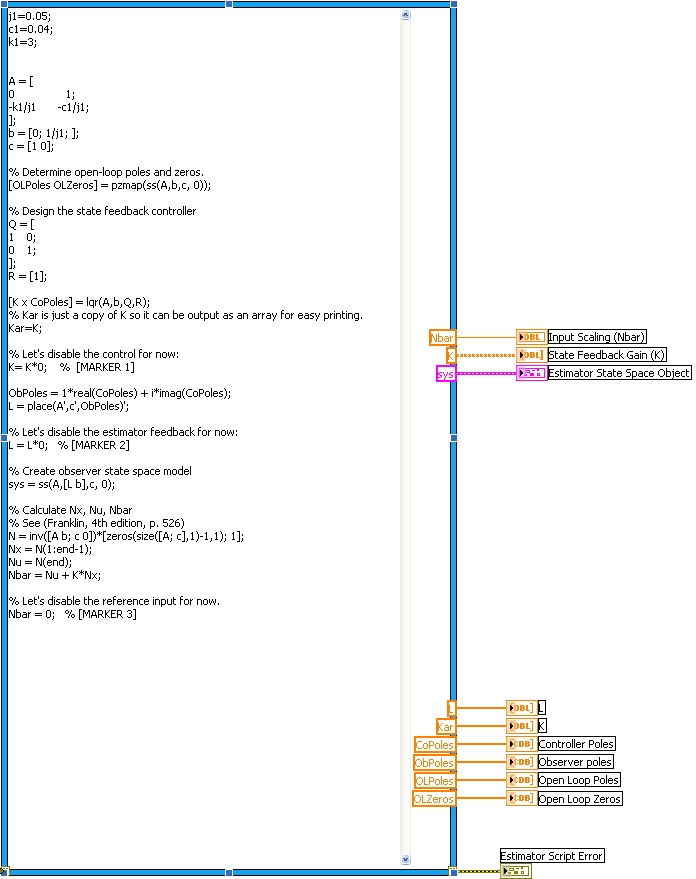
\includegraphics[width=6in]{statedomain/statespaceest}
\caption{State Space Estimation and Control}
\label{fig-SSestcontrol}
\end{figure}


%% Local Variables:
%% TeX-master: "../LVmanual.tex"
%% End:
